\documentclass[border=4pt]{standalone}
\usepackage{amssymb}
\usepackage{tikz}
\usetikzlibrary{arrows.meta,positioning,shapes.geometric,fit,calc,automata,trees}
\usepackage{float}
\usepackage{booktabs}
\usepackage{longtable}
\usepackage{array}
\usepackage[utf8]{inputenc}
\begin{document}

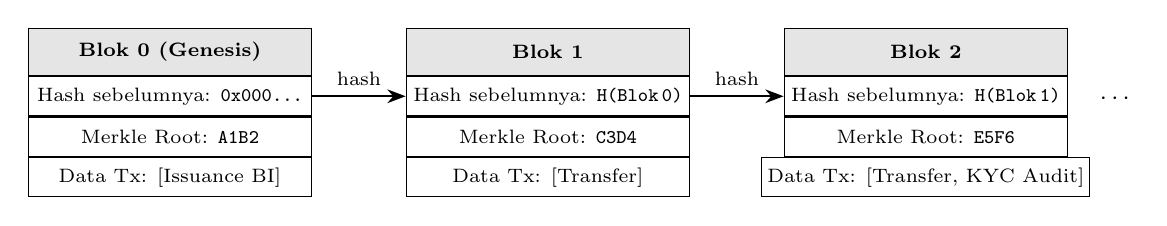
\begin{tikzpicture}[
  blkbody/.style={draw=black, fill=white, rectangle, minimum width=3.6cm,
    minimum height=0.5cm, align=center, font=\scriptsize, inner sep=2pt},
  blkhdr/.style={draw=black, fill=gray!20, rectangle, minimum width=3.6cm,
    minimum height=0.6cm, align=center, font=\scriptsize\bfseries, inner sep=2pt},
  ar/.style={-{Stealth}, thick},
]

%--- Blok 0 (Genesis) ---
\node[blkhdr] (b0h)  at (0, 0)     {Blok 0 (Genesis)};
\node[blkbody, below=0pt of b0h] (b0p) {Hash sebelumnya: \texttt{0x000\ldots}};
\node[blkbody, below=0pt of b0p] (b0m) {Merkle Root: \texttt{A1B2}};
\node[blkbody, below=0pt of b0m] (b0t) {Data Tx: [Issuance BI]};

%--- Blok 1 ---
\node[blkhdr] (b1h)  at (4.8, 0)   {Blok 1};
\node[blkbody, below=0pt of b1h] (b1p) {Hash sebelumnya: \texttt{H(Blok\,0)}};
\node[blkbody, below=0pt of b1p] (b1m) {Merkle Root: \texttt{C3D4}};
\node[blkbody, below=0pt of b1m] (b1t) {Data Tx: [Transfer]};

%--- Blok 2 ---
\node[blkhdr] (b2h)  at (9.6, 0)   {Blok 2};
\node[blkbody, below=0pt of b2h] (b2p) {Hash sebelumnya: \texttt{H(Blok\,1)}};
\node[blkbody, below=0pt of b2p] (b2m) {Merkle Root: \texttt{E5F6}};
\node[blkbody, below=0pt of b2m] (b2t) {Data Tx: [Transfer, KYC Audit]};

%--- Panah antar blok ---
\draw[ar] (b0h.east |- b1p.west) -- node[above,font=\scriptsize]{hash} (b1p.west);
\draw[ar] (b1h.east |- b2p.west) -- node[above,font=\scriptsize]{hash} (b2p.west);

\node[font=\small] at (12.0, -0.6) {$\cdots$};

\end{tikzpicture}%

\end{document}
